\section{Methodology}
\label{method}

The main goal of this research is to investigate the impact of atoms of confusion on JavaScript code comprehension. As such, in this paper we answer the following research questions: 

\begin{enumerate}[(RQ1)]
\item \rqa 
\item \rqb
% \item \rqc  
\item \rqd\castor{This one will probably be removed.}
\end{enumerate}


By answering these research questions, we can either generalize or refute the findings about atoms of confusion already discussed in the literature (goal of research questions (RQ1) and (RQ2)). In addition, answering the third question allows us to enrich existing catalogs about atoms of confusion and discuss how often they occur in practice\castor{This should probably be removed.}. Answering these research questions also lays the foundations for the implementation of tools that can automatically transform code into cleaner versions.
%---though we postpone these results to future research work.
We conduct a mixed-methods study to answer these questions. It includes two independently designed and conducted experiments\castor{I would rather use the term ``experiment''.}: a replication of the first study on atoms of confusion, but targeting JavaScript programs, and a new study using a latin square counterbalancing experimental design to control for subject experience. 
These two experiments explore the impact of atom candidates on understanding JavaScript code (goal of research question RQ1). They investigate whether or not programs that contain atom candidates produce a higher misunderstanding rate when programmers try to predict their outcome.\castor{I've removed the part about time because, in order for the first study to be a replication, we need to compute time differently, accounting for incorrect responses as well.}% and (b) require more time for programmers to predict their output. 
We leverage two independently-developed studies with different designs to more rigorously verify the impact of atoms of confusion in code comprehension activities. 
We also conduct a set of interviews with developers to contrast the quantitative results of the experiments with their preferences and opinions (thus addressing RQ2). 

\subsection{Replication Study Setting}\label{sec:meth:replication}

We call the first study we perform the \textit{``Replication Study''} because it is a partial replication~\cite{Juristo2012} of the first study on atoms of confusion, conducted by Gopstein et. al~\cite{DBLP:conf/sigsoft/GopsteinIYDZYC17}, but targeting JavaScript instead of the C language. Gopstein et. al. employ a randomized, partial counterbalancing experimental design on a sample of 73 subjects, mostly students, with three or more months of experience in C or C++. The control variable consists of a tiny program containing a single atom candidate and the treatment a functionally-equivalent version that does not contain the atom. The main dependent variable is whether subjects are able to correctly determine the output of the programs. The other dependent variable is the time required to correctly vs. incorrectly determine the outputs. The study has the null hypothesis that \textit{``code from both control and treatment groups can be hand-evaluated with equal accuracy''} and the alternate hypothesis that \textit{``the existence of an atom of confusion causes more errors than other code in hand-evaluated outputs.''}. For each atom candidate, six programs were built, three versions including the atom candidate and three versions not including it. Each subject is exposed to four programs for every atom candidate, two including an atom and two not including an atom.  

\subsubsection*{Experimental design} 

In this study we adopt the same experimental design, control and treatment variables, dependent variable, and hypotheses. We have also built six programs for each atom candidate, three with and three without the atom. Considering the elements that can vary in a replication study, defined by Juristo and Gomez~\cite{Juristo2012}, in this study we employ the same experimental protocol and construct operationalizations. We have different population properties, experimenters, and a different site. In addition, since we focus on a different language, some atoms that exist in C cannot by construction exist in JavaScript programs. Conversely, JavaScript exhibits atom candidates that do not exist in C. 

The design of the replication study considers two treatments: the presence or absence of atoms candidates within the programs. To identify atom candidates, we start out by selecting every atom candidate from Gopstein's study that can also happen in JavaScript. That excludes atoms related to pointers and preprocessor directives. Furthermore, we conduct an informal search of programming forums, solutions to Code Golf~\footnote{https://codegolf.stackexchange.com/} problems, code style guidelines, and expert knowledge to identify new atom candidates. Overall, the replication study analyzes 24 atoms, 15 from the original study and 9 that are new and specific to JavaScript. Table~\ref{tab:atoms_replication} presents the complete list. 

For each atom candidate, we write six short programs, three including and three not including the atom candidate. The former are the control for the study, or the obfuscated versions of the programs. The alternative, atom-free, versions of the programs are the treatment, or clean, versions. Each subject is exposed to one obfuscated and one clean version of each atom, totalling 48 programs, and should determine their outputs. As mentioned before, we measure answer correctness and the time to answer questions correctly vs. incorrectly. We control for learning effects~\cite{Neely:1991:SPE} in three manners. First, by having multiple obfuscated and clean versions for each atom and presenting only one of each per subject. Second, by presenting the programs in a random order. Third, by presenting obfuscated and clean versions corresponding to the same atom candidate with at least 11 other programs in between, in  accordance to the original experimental protocol~\cite{DBLP:conf/sigsoft/GopsteinIYDZYC17}. 

\subsubsection*{Study instrument} 

The study is conducted by means of a web application. As part of this effort, we carried out an informal pilot whose main objectives were (i) to spot bugs in the application and in the data collection mechanism; (ii) to gain feedback from respondents about the user experience of the application; and (iii) to formulate an estimate about how long answering the survey would take on average. Based on the feedback of the participants of the pilot, we present only one obfuscated and one clean version of each atom candidate, to reduce to total time of the study and potentially increase participation.% Initially, our plan was to present two of each. 

We organize the study in three sections. In the first one we present instructions and also a check button whose checking means users agree that all collected data will be used anonymously and solely for research purposes. The instructions explain how the survey works and asks them to dedicate their attention to it.  We stress to participants the importance of not using any aids during the survey, such as online or console interpreters. 

The second section presents the programs, one at a time. For each one, there is a text box where the answer should be written and a ``Next'' button. If the subject leaves the text box empty and presses ``Next'', this is treated as a wrong answer. To reduce the likelihood of a subject attempting to execute the programs, the web application verifies whether the subject tries to change tabs or windows and presents a pop-up message if that is the case. Furthermore, it presents the programs as images, instead of text. Upon submitting an answer for a particular program, the subject is automatically led to a similar page, containing the next one.

We do not provide feedback about the time subjects take to answer each question. We also do not tell them whether their answers are correct or not. This aims at avoiding introducing bias for future respondents. Since we posted the survey on social media platforms, possible threats could have arisen if we gave respondents instant feedback.


\subsubsection*{Study audience}

We posted the survey on the authors' social media platforms, on Brazilian CS departments' mailing lists, and on two programming subreddits. We explained our research purposes and asked developers to take the survey only if they have some familiarity with JavaScript. We collected 70 responses. The average survey respondent has a mean 26 months of experience in JavaScript, with a median of 12.\castor{We should not say this here unless we are able to do the same for the Latin square study. }


\subsection{Latin Square Study Setting}\label{sec:meth:survey}

This experiment uses a different experimental design that makes it possible to control for the experience of the subjects. For this study we employ a subset of the atom candidates used in the replication study. More specifically, we
%Since JavaScript and \clang have some constructs in common (Section~\ref{back}), we first 
select a set of 9+1 atom candidates: nine previously-validated atoms of confusion for the \clang language~\cite{DBLP:conf/sigsoft/GopsteinIYDZYC17} that also exist in JavaScript programs plus one atom candidate that is specific to the JavaScript language (Automatic Semicolon Insertion)\castor{I think the name of this atom is inconsistent between the studies}. 
Our supplementary material discusses and shows examples of the atoms we consider in our research.\castor{We should probably do this here or just refer to the table that I intend to insert for the replication study.}

\subsubsection*{Experimental design} 

The design of our second study blocks two variables (subject experience and the programs) and
considers two treatments: the presence or absence of atom candidates within the programs. 
To achieve such a design goal, controlling the effect of experience and individual programs, we resort to the \textit{Latin Square Design} \cite{Hunter-Experimenters}. Using this design we create a 2 x 2 matrix in which each row represents a subject and each column indicates the set of programs. The design of each square (a replica) is such that no treatment is repeated in the same row or column. For example, considering that we have a set of 10
code samples $s_0, s_1, ..., s_{10}$, if a given subject (P1) is asked to predict the output of the code samples $s_0, s_1, ..., s_5$ that contain atom candidates, then, when answering questions about clean programs, they will only be presented with clean versions of the code samples $s_6, s_7,..., s_{10}$. Furthermore, a given subject (P2), who constitutes the second row of our example square, will be asked questions about the clean versions for $s_1, s_2, ..., s_5$, and will answer questions about obfuscated programs for $s_6, s_7,..., s_{10}$. By doing that, we guarantee that all versions of the programs are contained within each square, and that each configuration occurs only once within a square. Figure \ref{fig:latinsquare} offers a visual representation of the concept.

  \begin{figure}[htb!]
      \noindent
      \centering
      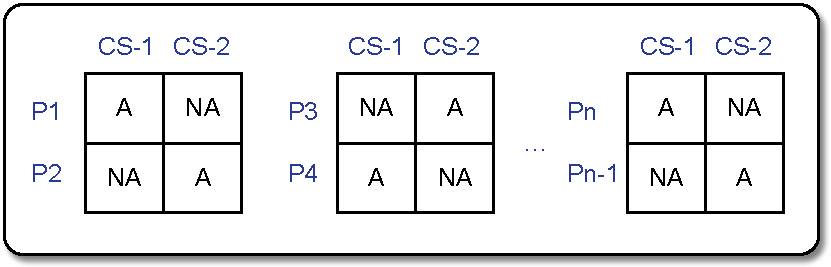
\includegraphics[scale=.50]{images/latin-square.pdf}
      \caption{Latin square design. Each ``square'' corresponds to 
      a replica in our study. Each replica comprises two participants (square rows, e.g., P1 and P2) 
      and two sets of programs (CS-1 and CS-2). We randomly apply the 
      treatments (atom or non-atom code) to the cells of the squares.} 
      \label{fig:latinsquare}
  \end{figure}

For each of the 10 selected atom candidates, we write one short program containing the atom. As in the replication study, we call them the obfuscated versions of the programs. We also write corresponding short programs without the atom candidates and call them the clean versions of the programs. Overall, the experiment employed 20 programs, 10 obfuscated and 10 clean. In order to reduce the cognitive effort, each subject was asked to predict the output of 10 programs, five obfuscated and five clean. The order in which they are presented is randomized. By doing this, we seek to minimize the chances of subjects being aware that the current listing they are analyzing contains (or not) atoms of confusion. That is, each subject should indicate what would be the outcomes of the programs, some of them having atoms of confusion (while other programs do not). Since participants are not exposed to obfuscated and clean versions corresponding to the same atom candidate, learning effect is not possible. We measure answer correctness and the total time each participant requires to participate in the experiment.

\subsubsection*{Study instrument} 

We implemented our survey as a web application and carried out a pilot, similarly to the replication study. 
%As part of this effort, we carried out an informal pilot whose main objectives were (i) to spot bugs in the application and in the data collection mechanism; (ii) to gain feedback from respondents about the user experience of the application; and (iii) to formulate an estimate about how long answering the survey would take on average.
Undergraduate students and professional colleagues took the pilot survey. Some users reported layout defects, and many reported that the landing page did not explain the survey well enough. We also spotted minor issues with our routines to create and populate the latin squares. 

We organize the survey in three sections. The first section aims to characterize the subjects, asking their age, education level, and programming experience. We also include a check button, whose checking means users agree that all collected data will be used solely for research purposes. In the second section, we present to the participants a small set of instructions, where we explain how the survey works and ask them to dedicate their attention to it. We stress to participants the importance of not using any aids during the survey, such as online or console interpreters. For each question page, we kept track of whether or not the subjects switch windows. 

The last section of the survey presents a sequence of ten questions, each containing a program. For each question, there is a text box where the answer should be written. There is also an ``I do not know'' button, which, when clicked, leads the subject to the next question. In our setting, ``I do not know'' is treated as a wrong answer. The programs are presented as images copied from a text editor, so as to demotivate respondents from resorting to external resources by copying and pasting the code into an interpreter. Upon submitting their answer for a particular question, the subjects are automatically led to a similar page, containing another program. Similarly to the replication study, we do not provide feedback about time and correctness to the subjects.


% \rb{nao acho esse paragrafo necessario} 
% \adriano{o de baixo ne? eu tambem acho}

% As we mentioned before, we first wrote the code listings in a text editor, and took pictures of it. In the case of an atom of confusion that was exclusive to JavaScript, which we called \textit{Automatic Semicolon Insertion} (see Appendix~\ref{sec:appendix-atoms}), it was necessary to remove the syntax highlighter. Even though semicolons at the end of statements are optional to programmers in JavaScript, the interpreter automatically inserts them into the code. Our text editor was incorrectly highlighting a line break after a return statement, even thought it was valid JavaScript syntax. We had thus to turn the highlighter off to take the picture of this atom. 

\subsubsection*{Study audience}

%% \diego{Esses detalhes são possíveis candidatos para remoção, se precisarmos de espaço}
%% {\color{blue}We invited developers to answer our survey by sending invitations to communities of JavaScript programmers on the Internet. Our initial plan was to try to engage contributors for two major JavaScript projects, namely Node.js and NPM. None of the projects, though, offered a direct way to interact with the community, such as an online discussion forums or mailing list. We would be required to first make contact with the projects' leaders, and only then would we have a chance to approach potential respondents. Due to time constraints, we decided to look for respondents elsewhere.}

We posted the survey on a JavaScript Reddit channel.\footnote{https://www.reddit.com/r/javascript/} We explained our research purposes and asked developers of any level of expertise to take the survey. Within twelve hours, we collected more than 150 answers, populating more than 70 replicas of the Latin Squares. We collected significant data on time taken and discrepancies in answer correctness between obfuscated and clean versions of the programs. Some inconsistencies arose while building the squares, for instance, when a user quit in the middle of the survey. We discarded from our study all squares that contained incomplete rows (a common approach for data imputation).
%Since we had a large enough number of samples, the squares we had to discard did not impact our analysis.

 
\subsection{Interview Study Setting}

To complement the two experiments, we perform semi-structured interviews with professional JavaScript developers, aiming to identify their perceptions regarding programs containing atoms of confusion (research question RQ2). We also ask each participant if they know of any other JavaScript-specific construct or idiom that they regard as being likely to make the code hard to understand.% (research question RQ3). 
In this section we detail the protocol we followed to conduct the interviews and to analyze the results.

% Nós realizamos entrevistas semi-estruturas com o objetivo de identificar a percepção dos desenvolvedores com experiência em JavaScript sobre algumas questões relacionadas à compreensão de código em JavaScript. Assim, nesta Seção nós descrevemos os procedimentos adotados para selecionar os participantes para as entrevistas e detalhamos como as entrevistas foram conduzidas. Além disso, detalhamos como os resultados das entrevistas foram analisados.

\subsubsection*{Participant Selection} We invite the participants of the interviews using a snowballing technique. That is, starting from our network of contacts, we invite an initial set of candidates to take part in our survey. From this initial list, we ask for an indication of additional candidates. Our main selection criterion is that all participants should have been working with JavaScript in their daily professional activities. We invite a total of 17 developers, and 15 of them agree to participate.   
%We conducted the interviews for a period of two weeks.


\subsubsection*{Interview Process} We conduct semi-structured interviews using web conferencing software. We record all the interviews with the consent of the participants. On average, the interviews last 26.29 minutes, with the shortest one lasting 14.59 minutes and the longest one 43.06 minutes. 
Two of the researchers conduct the interviews, and a third one listens to all the recordings to cross-validate the collected data.
The interviews have three main parts. In the first one, we ask the developers the following demographic information: name, email, gender, level of education, current job position, JavaScript experience in years, and other programming languages they have worked with.
Table \ref{pinterview} summarizes this demographic information.

\begin{table}[htb!]
  \centering
  \caption{Demographic information of the participants}
\begin{scriptsize}  
\begin{tabular}{clcl}
\toprule
ID & Education & JS Experience & Other Languages \\ \midrule 
P1 & BSc Degree & 9 years & Java, PHP, C, Go  
\\ 
P2 & HS Degree & 3 years & Python, Go, Dart, Lua, C++, C\#
\\ 
P3 & BSc Degree & 4 years & Java, C
\\ 
P4 & Undergraduate & 3 years & Python, C, C++, Java, Go
\\ 
P5 & Master Student & 3 years & Python, SQL
\\ 
P6 & Bsc Degree & 15  years  & Java, PHP, C, Python , Ruby, C\#
\\ 
P7 & BSc Degree  & 6 years & C, C++, Java, Assembly, Kotlin
\\ 
P8 & PhD Degree & 2 years & Java, Python
\\ 
P9 & BSc Degree  & 5 years & PHP
\\ 
P10 & Master Student & 4 years & Java, C\# and Python
\\ 
P11 & Master Student & 4 years & Java, Erlang, C\#, Cobol
\\ 
P12 & Master Degree & 1 year & C
\\ 
P13 & Master Degree & 13 years & Java, PHP
\\ 
P14 & Master Student & 3 years & C, Python, Ruby
\\ 
P15 &  BSc degree  & 2 years & Java, PHP
\\ \bottomrule
\end{tabular}
\end{scriptsize}
    \label{pinterview}
\end{table}

In the second part of the interview our aim is to allow the subjects to describe their JavaScript experience, as well as to allow them to reveal any JavaScript constructs they regard as innately confusing. This allows us to identify potential atom candidates that are more specific to the JavaScript language. Examples of questions we explore in this section include: \emph{Does JavaScript favor developers to produce code that is hard to understand?} and \emph{Do you regard any particular construct or idiom of the language as especially confusing?}

In the third part of the interview, participants are shown pairs of programs that were used in the first study, where each pair contains a clean and an obfuscated version of the same atom candidate. The participants 
%were told both sides of each pair had the same output, and 
are asked to evaluate which version of the code is easier to understand. To avoid introducing bias in the answers, the interviewers do not explain that one of the versions in each pair contains the atom under investigation. Subjects are just presented the pairs of programs and allowed to take the necessary time to decide on the most readable one.

\subsubsection*{Interview Analysis}

We first transcribe each interview and then examine the broad distribution of the answers. Our goal is to build an initial understanding of the participants' perceptions with regards to the challenges to understand JavaScript code in general and JavaScript code with atoms of confusion in particular. We follow-up with an open-coding procedure, highlighting the main themes and quoting the answers of the participants. We present these results in Section~\ref{sec:interview-results}. 
%Finally, we consolidate the feedback of the participants with respect to the confusion that our set of atom candidates might introduce in JavaScript code.

%\subsection{Third Study: Additional Survey and Interviews}

% \rb{acho que aqui podemos incluir o segundo survey e a segunda
%  rodada das entrevistas, explorando os \'{a}tomos adicionais}


\subsection{Mining JavaScript Software Repositories Setting}

To understand how often the analyzed atom candidates appear in open source projects, and thus answer our fourth research question (\emph{What is the frequency of occurrence of atoms of confusion in practice?}), we mined a set of GitHub open source repositories. To this end, we first collected the most popular GitHub repositories that are primarily written in JavaScript. We measured popularity using the project's stargazers. This metric, available through the GitHub API, represents the number of stars a project received from users of the platform. The same metric has been used in a number of previous studies as a proxy to estimate a project's popularity~\cite{gyimesi2019bugsjs,canedo:esem2020}. We then selected the top 100 most popular repositories and removed projects that did not reach the first quartile of the distribution of lines of code.

After filtering out JavaScript project candidates, in the second step we built a curated dataset comprising the top \minedprojects repositories. Examples of projects in this dataset include \textsc{React}, \textsc{Node JS}, and \textsc{AngularJS}. Table~\ref{tab:projects-statistics} presents some statistics about the projects we consider in our research. The size of the projects range from small ones (5543 lines of code) to complex systems with more than 1 MLOC. All projects in our dataset have at least \num{1244} forks and at least \num{23672} stars. We automated all the steps to filter, clone, and collect the statistics from the repositories using Python scripts.

We mined the occurrence of atom candidates from the repositories in our curated dataset using source code queries that we wrote using the CodeQL language~\cite{moor:gttse2007}. CodeQL is an object-oriented variant of the Datalog language~\cite{rodriguez2020efficient}, and currently supports researchers and practitioners to query the source code of systems written in different languages (such as \cpplang, Java, and JavaScript). We also automate the process of running the queries and exporting the results to a format that simplifies our analysis (and also the reproduction of this study). Finally, we computed some descriptive statistics to measure the prevalence of atoms of confusion in practice. 

\begin{table}[ht]
  \centering
   \caption{Some descriptive statistics about the projects used in the MSR study}
  \begin{scriptsize}
 \begin{tabular}{rrrrr}
   \hline
                       & Min.             & Median        & Mean             & Max. \\ \hline
 Lines of Code         & \num{5543}       & \num{36161.5} & \num{111432.33}  & \num{1278405} \\
 Num. of Forks         & \num{1244}       & \num{6078}    & \num{8906.24}    & \num{68849} \\
 Num. of Contributors  & \num{6}          & \num{285.5}   & \num{533.44}     & \num{4047} \\
 Num. of Stars         & \num{23672}      & \num{34990}   & \num{46919.51}   & \num{310935} \\
 
    \hline
 \end{tabular}
 \end{scriptsize}
 \label{tab:projects-statistics} 
 \end{table}


